\documentclass[10pt, a4paper]{arbeitsblatt}

\ladeModule{theme,boxen,tabellen}
\ladeFach[]{informatik}

\aboptionen{
	name		= {J. Neugebauer},
	kuerzel		= {Ngb},
	titel		= {Telnet},
	reihe		= {Rechnernetze},
	fach		= {Informatik},
	lerngruppe	= {Q2},
	nummer		= {II.05},
	lizenz		= {cc-by-nc-sa-4},
	version		= {2022-01-09},
}

\begin{document}
\ReiheTitel

Ein \emph{Telnet-Client} ist ein Programm, mit dem Verbindungen zu Servern hergestellt werden können. Auf fast jedem Betriebssystem gibt es einen \emph{Telnet-Client}. Unter Windows startet man zum Beispiel eine Kommandozeile (\enquote{\textsc{Start}} $\rightarrow$ \code{cmd} $\rightarrow$ \keys{ENTER}) und gibt den Befehl \code{telnet} gefolgt von einer \emph{IP-Adresse} oder einem \emph{Hostnamen} und einer \emph{Portnummer} ein. Telnet kommuniziert also über eine \emph{TCP-Verbindung}.

Um zum Beispiel eine Verbindung zum Google-Server über den Port 80 (HTTP) aufzubauen, gibt man ein:

\begin{center}
	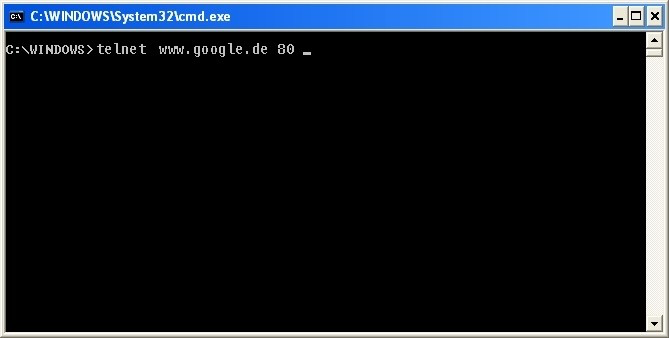
\includegraphics[width=.8\textwidth]{Q2-GK-AB.II.5-Abb_cmd.png}
\end{center}

Nun werden \textbf{alle} Eingaben (bei betätigen von \keys{ENTER}) an den Server geschickt. Alle Eingaben heißt, dass auch Tasten wie \keys{Backspace}, oder \keys{$\leftarrow$} (\enquote{\textsc{Pfeil links}}) übertragen werden. Die Eingabe

\begin{verbatim}
	HELLO
\end{verbatim}

ist also etwas anderes als die Eingabe

\begin{verbatim}
	HELLL<Backspace>O
\end{verbatim}

bei der man das überflüssige \enquote{L} vor dem abschicken wieder löscht. Manche Server können mit diesen \enquote{fehlerhaften} Eingaben umgehen, manche leider nicht.

Um eine Verbindung zu einem anderen Programm auf dem gleichen Rechner herzustellen kann die lokale IP \code{127.0.0.1} genutzt werden:

\begin{center}
	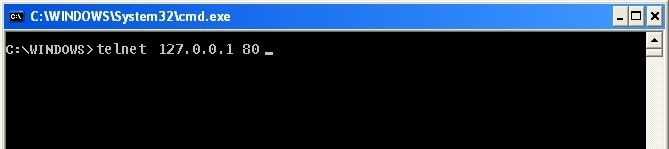
\includegraphics[width=.8\textwidth]{Q2-GK-AB.II.5-Abb_home.png}
\end{center}

\newpage

\begin{aufgabe}[icon=\iconComputer]
Verbinde dich zu einem Webserver mit einem beliebigen Hostnamen (zum Beispiel \enquote{neugebauer.cc}, \enquote{ngb.schule}, \enquote{google.com} oder \enquote{whitehouse.gov}) und über den Port 80.

Du bist nun wie ein Browser mit dem Server verbunden und kannst über das \emph{HTTP-Protokoll} mit ihm kommunizieren. Die folgenden Befehlsfolge zeigt ein Beispiel, wie eine Webseite abgerufen werden kann:

\textbf{\code{telnet jonas-neugebauer.de 80}}\\
{\color{gray}
\verb|Trying 2a00:1158:1000:300::5f2...| \\
\verb|Connected to neugebauer.cc.|\\
\verb|Escape character is '^]'.|
}

\textbf{\code{GET /index.html HTTP/1.1}} \\
\textbf{\code{host: jonas-neugebauer.de}}

Informiere dich über das \emph{HTTP-Protokoll} und besonders das \code{GET}-Kommando. Probier dann verschiedene Kombinationen von Parametern für das \code{GET}-Kommando aus (versuch statt \enquote{/index.html} doch mal \enquote{/images/avatar.jpg} vom Host \enquote{jonas-neugebauer.de} abzurufen).
\end{aufgabe}

\begin{aufgabe}[icon=\iconComputer]
	Im Tauschordner findest du im Ordner \ordner{Server} verschiedene Server-Programme. Probiere sie aus, indem du eins startest und zum angezeigten Port verbindest:

	\code{telnet 127.0.0.1 <PORTNUMMER>}

	Probiere dann aus, verschiedene Nachrichten zu senden und herauszufinden, wie der Server funktioniert.

	\hinweis{Du kannst den Server auch auf einem anderen Rechner starten und statt zu \code{127.0.0.1} zur IP des Servers verbinden. Dazu musst du auf der Server-Maschine zunächst die IP mit dem \code{ipconfig}-Kommando ermitteln.}

	\paragraph{Hinweise zum TicTacToe-Server:}
	Verbinde zum Port 1000: \code{telnet 127.0.0.1 1000}

	Es sind folgende Befehle erlaubt:

	\begin{tabularx}{\textwidth}{|l|X|}\hline
	\code{BOARD} & Zeigt das aktuelle Spielfeld und den Spielzustand an. \\\hline
	\code{RESTART} & Startet ein neues Spiel. \\\hline
	\code{NAME <name>} & Setzt zu Beginn den Nickname. \\\hline
	\code{SET <x>,<y>} & Setzt bei den Koordinaten \textsc{(x | y)} ein Kreuz. \\\hline
	\end{tabularx}

	Versuch ein Spiel komplett über \programm{telnet} zu spielen.
\end{aufgabe}

\begin{aufgabe}[icon=\iconComputer]
	Wird kein Port angegeben, dann wird standardmäßig der Port 23 benutzt. Eine Verbindung kann entweder mit einem der Kommandos \code{exit} oder \code{quit} beendet, oder mit der Tastenkombination \keys{Strg+C} abgbrochen werden.

	Probiere \programm{telnet} Verbindungen zu einigen der folgenden Servern aus:

	\begin{itemize}
		\item \enquote{telehack.com} (Probiere dann das Kommando \code{eliza} aus. \code{help} erklärt dir die verfügbaren Kommandos.)
		%\item \enquote{rainmaker.wunderground.com}
		\item \enquote{towel.blinkenlights.nl} (Viel Spaß, aber bitte nicht bis zum Ende anschauen \faGrinWink[regular])
		\item \enquote{aardmud.org} (siehe vorherigen Hinweis ...)
		\item \enquote{freechess.org}
		\item \enquote{mtrek.com} (Port 1701)
	\end{itemize}
\end{aufgabe}

\end{document}
